\documentclass[11pt]{amsbook}

\usepackage[turkish]{babel}
\usepackage{../Ceyhun}
\usepackage{../amsTurkish}

\begin{document}
\hPage{037}
\subsection{RAMSEY SAYILARI}
'Altı kişiden oluşan herhangi bir toplulukta, ya birbirini tanıyan ya da tanımayan en az 3 kişi vardır' yargısını tanıtlayabilir misiniz?

İşte bu soru, çizge kuramında \textit{Ramsey  sayısı} diye adlandırılan bir özelliğin çıkmasına neden olmuştur. Altı kişiden oluşan bir topluluktaki kişileri düğümler ve kişiler arasındaki tanışıklığı da ilgili düğümler arasındaki ayrıtlar ile gösterirsek, bu soruyu: '6 düğümden oluşan Ç çizgesinde ya da \c{\~C} tümlerçizgesinde en az bir üçgen olduğunu gösteriniz' diye de sorabiliriz. Örneğin, \reffig{fig:altiKisidenOlusanBirTopluluk}a daki çizgeyi düşünelim. Her ne kadar Ç de bir üçgen yoksa da, \reffig{fig:altiKisidenOlusanBirTopluluk}b de gösterilen \c{\~C} de bir çok üçgen vardır (\c{\~C}  de  bulunan üçgenleri sayınız). Bu durumun 6 düğümlü bütün çizgeler için geçerli 
\begin{figure}[h]
	\centering
	\includegraphics[width=0.9\textwidth]{images/ceyhun-037-fig01}
	\caption{Altı kişiden oluşan bir topluluk}
	\label{fig:altiKisidenOlusanBirTopluluk}
\end{figure}
\end{document}